\documentclass[11pt,oneside]{article}	%use"amsart"insteadof"article"forAMSLaTeXformat
\usepackage{geometry}		%Seegeometry.pdftolearnthelayoutoptions.Therearelots.
\geometry{letterpaper}		%...ora4paperora5paperor...
%\geometry{landscape}		%Activateforforrotatedpagegeometry
%\usepackage[parfill]{parskip}		%Activatetobeginparagraphswithanemptylineratherthananindent
\usepackage{graphicx}				%Usepdf,png,jpg,orepsßwithpdflatex;useepsinDVImode
								%TeXwillautomaticallyconverteps-->pdfinpdflatex		
\usepackage{amssymb}
\usepackage[colorlinks]{hyperref}

%----macros begin---------------------------------------------------------------
\usepackage{color}
\usepackage{amsthm}

\def\conv{\mbox{\textrm{conv}\,}}
\def\aff{\mbox{\textrm{aff}\,}}
\def\E{\mathbb{E}}
\def\R{\mathbb{R}}
\def\Z{\mathbb{Z}}
\def\tex{\TeX}
\def\latex{\LaTeX}
\def\v#1{{\bf #1}}
\def\p#1{{\bf #1}}
\def\T#1{{\bf #1}}

\def\vet#1{{\left(\begin{array}{cccccccccccccccccccc}#1\end{array}\right)}}
\def\mat#1{{\left(\begin{array}{cccccccccccccccccccc}#1\end{array}\right)}}

\def\lin{\mbox{\rm lin}\,}
\def\aff{\mbox{\rm aff}\,}
\def\pos{\mbox{\rm pos}\,}
\def\cone{\mbox{\rm cone}\,}
\def\conv{\mbox{\rm conv}\,}
\newcommand{\homog}[0]{\mbox{\rm homog}\,}
\newcommand{\relint}[0]{\mbox{\rm relint}\,}

%----macros end-----------------------------------------------------------------

\title{Boundary operators on LAR
\footnote{This document is part of the \emph{Linear Algebraic Representation with CoChains} (LAR-CC) framework~\cite{cclar-proj:2013:00}. \today}
}
\author{Alberto Paoluzzi}
%\date{}							%Activatetodisplayagivendateornodate

\begin{document}
\maketitle
\nonstopmode

\begin{abstract}
The various versions of boundary operators on Linear Algebraic Representation of cellular complexes are  developed in this module, in order to maintain under focus their proper development, including the possible special cases.
\end{abstract}

\tableofcontents
\newpage

\section{Introduction}

In the current \texttt{LarLib} implementation, we have to distinguish between between dimension-independent, dimension-dependent, signed and non-signed operators.
Therefore a code refactoring of \texttt{LarLib}---related to boundary/coboundary operators---started here, with the aim of both providing a precise mathematical definition within the LAR framework, and to simplify and generalise the implemented algorithms.


\section{Implementation}

We start this section by making a distinction between the (matrices of) boundary operators for the linear spaces $C_k$ of chains over the field $\Z_2 = \{0,1\}$ and over the field $\Z$ of integer numbers.
We call either \emph{non-signed} or \emph{signed} the corresponding boundary operators, respectively, since the matrix elements take values within the sets $\{-1,0,+1\}$ or $\{0,1\}$, correspondingly.
Of course, the associated matrices of \emph{coboundary} operators are their transpose matrices.


\subsection{Non-signed operators}

For several computations, the knowledge of the matrices of non-signed boundary operators is sufficient. 
Therefore we will use such tool wherever possible, since its computation is much faster in term of computing time. 

In the following we provide be binary operator matrices provided by two implementations,
respectively named \texttt{boundary} and \texttt{boundary1}. The first one works correctly only with convex cells; the second one works also with non-convex but path-connected cells.


\subsubsection{Dimension-independence}

As we show in the following, in order to compute the non-signed boundary operator $\partial_d$, it it sufficient to have knowledge of the $M_d$ and $M_{d-1}$ characteristic matrices of $d$-cells and their $(d-1)$-facets, at least in the case of cellular complexes with convex cells. Conversely, for more general non-convex but simply-connected cells, also the $M_{d-2}$ matrix is needed.

\paragraph{Convex-cells}

The algorithm used is pretty easy to present. The compressed characteristic matrices of $d$-cells and $(d-1)$-cells, denoted as \texttt{cells} and \texttt{facets}, respectively, are first put in \texttt{csr} format as \texttt{csrCV} and \texttt{csrFV}. Then the incidence matrix \texttt{csrFC} in compressed sparse row format is computed by matrix product of the compressed characteristic matrices. 

The element $(i,j)$ of this matrix provides the number of vertices in the intersection of \emph{facet} $i$ and \emph{cell} $j$, whereas the number of non-zero elements in each \texttt{csrFV} \emph{row} gives the number of vertices of the facet represented by the row, and is stored in \texttt{facetLengths}. 

The \texttt{boundary} function---to be used only with dimension-independent LAR convex cells---is written efficiently in the following script, by using only the standard functions and attributes of the \texttt{scipy.sparse} module.

The variable \texttt{facetCoboundary} stores in a list, for every facet (\texttt{for h in range(m)})
the list of cells in its \emph{coboundary}, to be stored in the output \texttt{csr\_matrix} boundary matrix as column indices of elements with non-zero (i.e.~$1$) value.

Notice that both the computation of \texttt{facetCoboundary} contents, and the output of the compressed boundary matrix, are performed in the most efficient way---according to the internal design of the scipy's \texttt{csr} sparse data structure.

%-------------------------------------------------------------------------------
@D convex-cells boundary operator
@{""" convex-cells boundary operator --- best implementation """
def boundary(cells,facets):
    lenV = max(CAT(cells))+1
    csrCV = csrCreate(cells,lenV)
    csrFV = csrCreate(facets,lenV)
    csrFC = csrFV * csrCV.T
    facetLengths = [csrFacet.getnnz() for csrFacet in csrFV]
    m,n = csrFC.shape
    facetCoboundary = [[csrFC.indices[csrFC.indptr[h]+k] 
        for k,v in enumerate(csrFC.data[csrFC.indptr[h]:csrFC.indptr[h+1]]) 
            if v==facetLengths[h]] for h in range(m)]
    indptr = [0]+list(cumsum(AA(len)(facetCoboundary)))
    indices = CAT(facetCoboundary)
    data = [1]*len(indices)
    return csr_matrix((data,indices,indptr),shape=(m,n),dtype='b')
@}
%-------------------------------------------------------------------------------


\paragraph{Non-convex LAR cells}

A more general \texttt{boundary1} operator is given in the following, aiming at compute the boundary matrix for general non-convex cellular decompositions, including \emph{multiply connected} LAR models.
Notice that in this case an input triple made by \texttt{CV}, \texttt{FV}, and \texttt{EV} is needed,
where---more in general embedded in $\mathbf{E}^d$---they stand for the (binary compressed) characteristic matrices $M_d$, $M_{d-1}$, and $M_{d-2}$.

First the \texttt{boundary} operator for the convex case is computed within the \texttt{out} variable of \texttt{csr\_matrix} type. Then every \texttt{out} row (i.e.~every $(d-1)$-facet of the $d$-complex) is tested for \emph{reliability}, since every $(d-1)$-face can be shared by \emph{at most two} $d$-cells in a $d$-complex . When this condition is not satisfied, deeper tests are needed to understand what row elements must be forced to value 1, since the $(d-1)$-face itself is a subset, but not actually a facet, of the corresponding $d$-cell. 

In presence of some ``unreliable'' facets, the matrix \texttt{csrBBMat} of the operator $\partial_{d-1}\circ\partial_d$ and the relation \texttt{FE} between faces of dimensions $d-1$ and $d-2$ are computed. Now, let us notice that the columns of \texttt{csrBBMat} report the number of incidences of the $d-2$ faces (as belonging to $(d-1)$-facets embedded on the boundary) and $d$-cells (that are associated to such matrix columns). Hence, in a regular (convex) $d$-complex, such numbers are always even, and in $\Z_2$ arithmetic are reduced to zero, in order to satisfy the fundaments equation $\partial\partial=0$. 

Conversely, with non-convex LAR cells, some incidence numbers may get odd values, due to the non-strict coincidence between cell facets and vertex subsets.
Therefore, for ``unreliable'' $h$ rows (facets) the \texttt{csrBBMat} columns tracked by ones in $[\partial_d]$ are checked, looking for elements of $(h,k)$ indices with value greater that 2.

%-------------------------------------------------------------------------------
@D path-connected-cells boundary operator
@{""" path-connected-cells boundary operator """
import larlib
import larcc
from larcc import *

def csrBoundaryFilter1(unreliable,out,csrBBMat,cells,FE):
    for row in unreliable:
        for j in range(len(cells)):
            if out[row,j] == 1:
                cooCE = csrBBMat.T[j].tocoo()
                flawedCells = [cooCE.col[k] for k,datum in enumerate(cooCE.data)
                    if datum>2]
                if all([facet in flawedCells  for facet in FE[row]]):
                    out[row,j]=0
    return out

def boundary1(CV,FV,EV):
    out = boundary(CV,FV)
    def csrRowSum(h): 
        return sum(out.data[out.indptr[h]:out.indptr[h+1]])    
    unreliable = [h for h in range(len(FV)) if csrRowSum(h) > 2]
    if unreliable != []:
        csrBBMat = boundary(FV,EV) * boundary(CV,FV)
        print "\ncsrBBMat =",csrBBMat.todense(),"\n"
        lenV = max(CAT(CV))+1
        FE = larcc.crossRelation(lenV,FV,EV)
        out = csrBoundaryFilter1(unreliable,out,csrBBMat,CV,FE)
    return out
@}
%-------------------------------------------------------------------------------



%-------------------------------------------------------------------------------
@D From cells and facets to boundary cells
@{def totalChain(cells):
    return csr_matrix(len(cells)*[[1]])

def boundaryCells(cells,facets):
    csrBoundaryMat = boundary(cells,facets)
    csrChain = csr_matrix(totalChain(cells))
    csrBoundaryChain = csrBoundaryMat * csrChain
    for k,value in enumerate(csrBoundaryChain.data):
        if value % 2 == 0: csrBoundaryChain.data[k] = 0
    out = [k for k,val in enumerate(csrBoundaryChain.data.tolist()) if val == 1]
    return out

def boundaryCells1(cells,facets,faces):
    csrBoundaryMat = boundary1(cells,facets,faces)
    csrChain = csr_matrix(totalChain(cells))
    csrBoundaryChain = csrBoundaryMat * csrChain
    """
    for k,value in enumerate(csrBoundaryChain.data):
        if value % 2 == 0: csrBoundaryChain.data[k] = 0
    """
    out = [k for k,val in enumerate(csrBoundaryChain.data.tolist()) if val == 1]
    return out
@}
%-------------------------------------------------------------------------------



\subsection{Signed operators}


\section{Exporting}

%-------------------------------------------------------------------------------
@O larlib/larlib/boundary.py
@{""" boundary operators """
from larlib import *
@< convex-cells boundary operator @>
@< path-connected-cells boundary operator @>
@< From cells and facets to boundary cells @>
@}
%-------------------------------------------------------------------------------


\section{Testing}

\section{Non-signed operators}

\paragraph{Correct boundary extraction example}

The \texttt{boundary.boundary()} operator is applied here to a cellular 2-complex of convex cells, producing correct result.

%-------------------------------------------------------------------------------
@O test/py/boundary/test01.py
@{""" testing boundary operators (correct result) """
from larlib import *

filename = "test/svg/inters/boundarytest0.svg"
lines = svg2lines(filename)
VIEW(STRUCT(AA(POLYLINE)(lines)))
    
V,FV,EV,polygons = larFromLines(lines)
VV = AA(LIST)(range(len(V)))
submodel = STRUCT(MKPOLS((V,EV)))
VIEW(larModelNumbering(1,1,1)(V,[VV,EV,FV],submodel,0.2))
VIEW(EXPLODE(1.2,1.2,1.2)(MKPOLS((V,[EV[e] for e in boundaryCells(FV,EV)],))))
VIEW(EXPLODE(1.2,1.2,1.2)(MKTRIANGLES((V,FV,EV))))

boundaryOp = boundary1(FV,EV,VV)

for k in range(1,len(FV)+1):
    faceChain = k*[1]
    BF = chain2BoundaryChain(boundaryOp)(faceChain)
    VIEW(STRUCT(MKPOLS((V,[EV[e] for e in BF]))))
@}
%-------------------------------------------------------------------------------

\paragraph{Wrong boundary extraction example}

The \texttt{boundary()} operator, applied  to a cellular 2-complex wih some non-convex cells, produces incorrect results. In such cases a correct result may be produced only by chance (sometimes this happens). So, be careful to use it only when the precondition (of cell convexity) is everywhere verified. In order to get always a correct result, use the \texttt{boundary1} operator.

%-------------------------------------------------------------------------------
@O test/py/boundary/test02.py
@{""" testing boundary operators (wrong result) """
from larlib import *

#filename = "test/svg/inters/boundarytest3.svg" # KO (MKTRIANGLES) with boundarytest3 !!!
filename = "test/svg/inters/boundarytest4.svg"
lines = svg2lines(filename)
VIEW(STRUCT(AA(POLYLINE)(lines)))
    
V,FV,EV,polygons = larFromLines(lines)
VV = AA(LIST)(range(len(V)))
submodel = STRUCT(MKPOLS((V,EV)))
VIEW(larModelNumbering(1,1,1)(V,[VV,EV,FV],submodel,0.2))

boundaryOp = boundary1(FV,EV,VV)  # <<======  NB
#boundaryOp = boundary(FV,EV)  # <<======  NB
BF = chain2BoundaryChain(boundaryOp)([1]*len(FV))

VIEW(EXPLODE(1.2,1.2,1.2)(MKPOLS((V,[EV[e] for e in BF])))) 
VIEW(EXPLODE(1.2,1.2,1.2)(MKFACES((V,FV,EV)))) 
VIEW(SKEL_1(EXPLODE(1.2,1.2,1.2)(MKTRIANGLES((V,FV,EV))))) 

for k in range(1,len(FV)+1):
    faceChain = k*[1]
    boundaryChain = chain2BoundaryChain(boundaryOp)(faceChain)
    VIEW(STRUCT(MKPOLS((V,[EV[e] for e in boundaryChain]))))
@}
%-------------------------------------------------------------------------------

\begin{figure}[htbp] %  figure placement: here, top, bottom, or page
   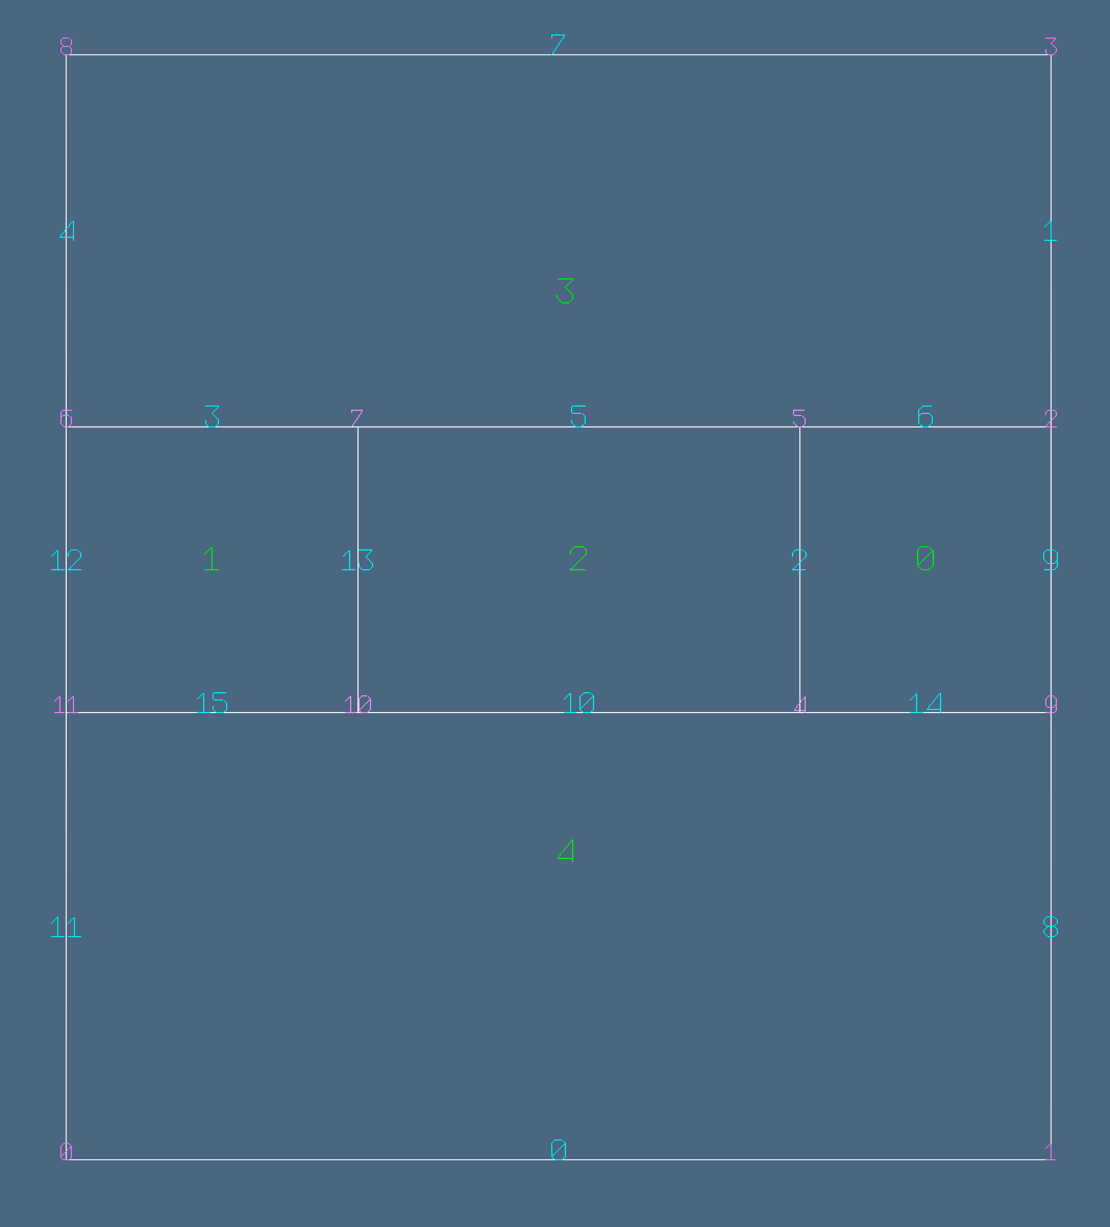
\includegraphics[height=0.245\linewidth,width=0.245\linewidth]{images/boundary-test01-2} 
   
\includegraphics[height=0.245\linewidth,width=0.245\linewidth]{images/boundary-test01-3} 
   
\includegraphics[height=0.245\linewidth,width=0.245\linewidth]{images/boundary-test01-4} 
   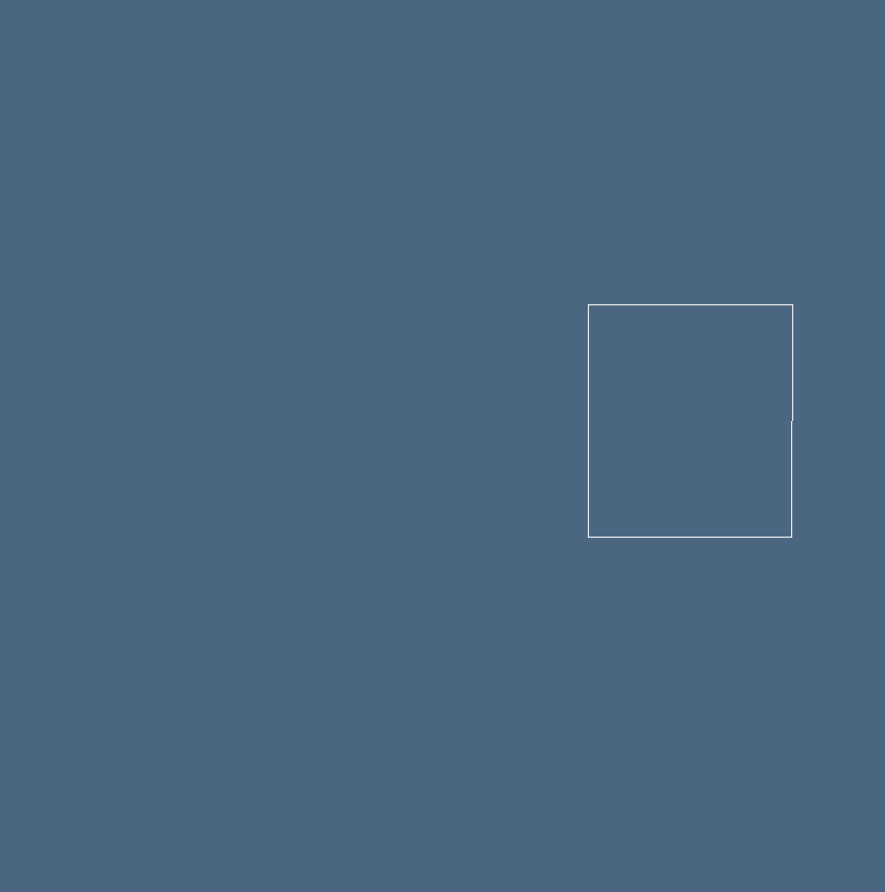
\includegraphics[height=0.245\linewidth,width=0.245\linewidth]{images/boundary-test01-5} 

   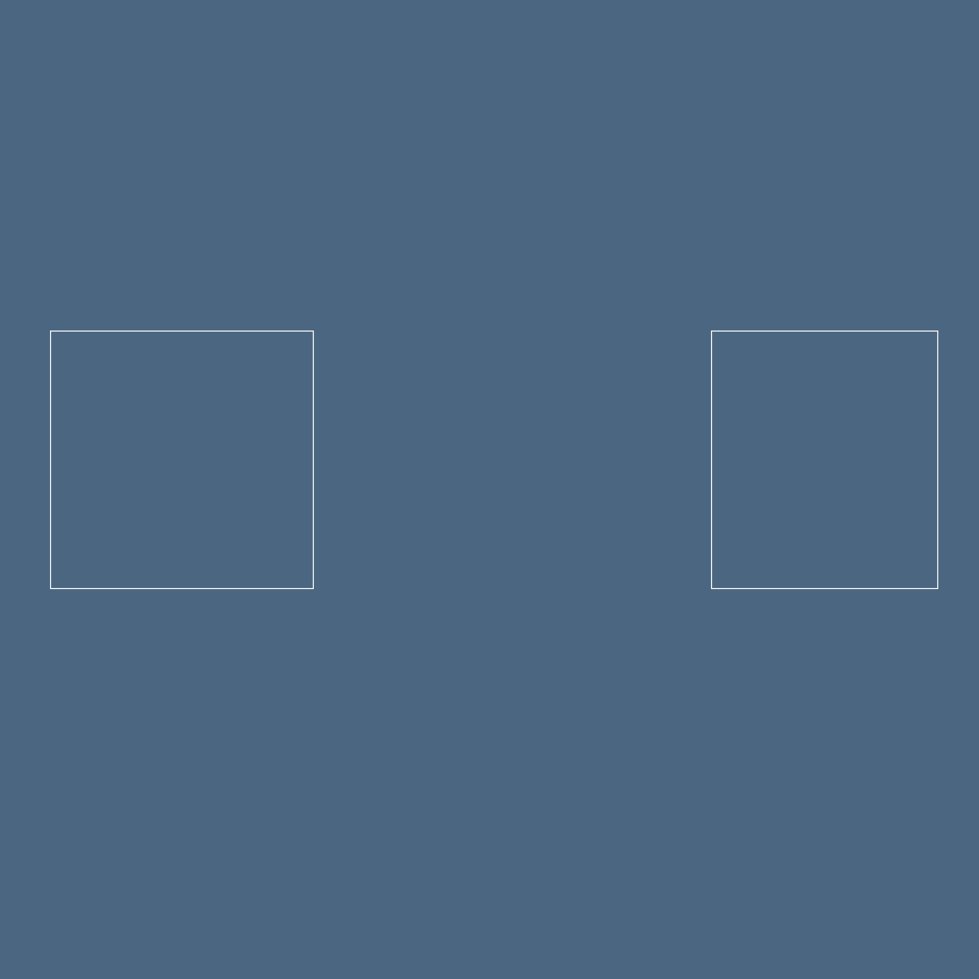
\includegraphics[height=0.245\linewidth,width=0.245\linewidth]{images/boundary-test01-6} 
   
\includegraphics[height=0.245\linewidth,width=0.245\linewidth]{images/boundary-test01-7} 
   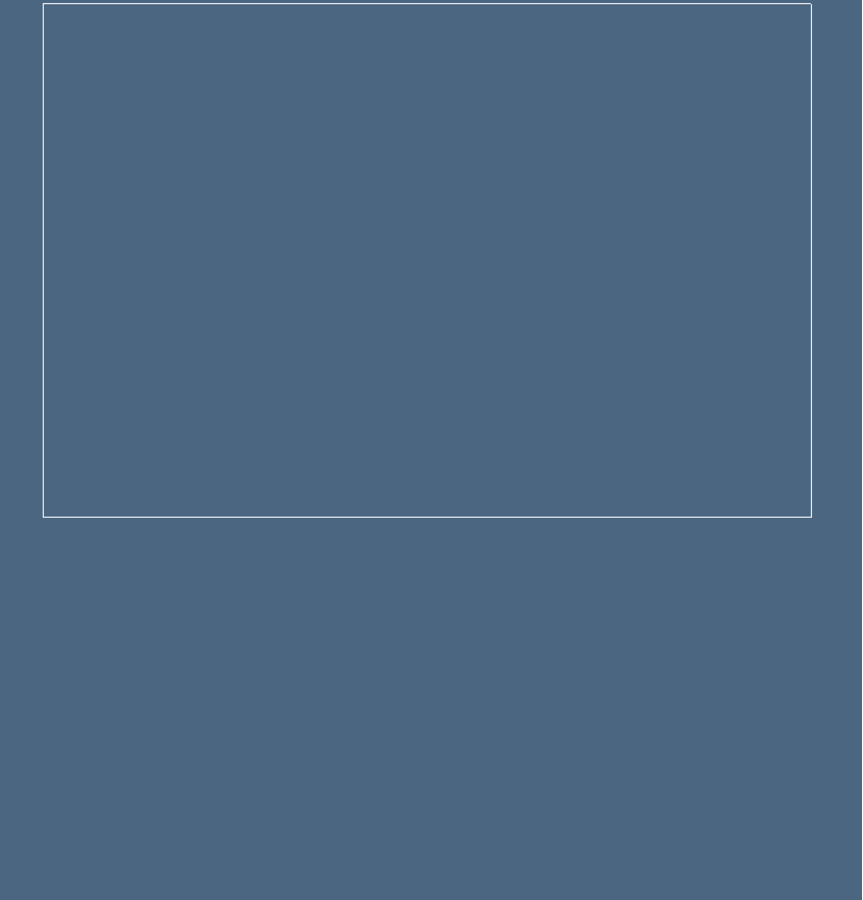
\includegraphics[height=0.245\linewidth,width=0.245\linewidth]{images/boundary-test01-8} 
   
\includegraphics[height=0.245\linewidth,width=0.245\linewidth]{images/boundary-test01-9} 
   \caption{Convex-cell 2-complex. (a) Indexing of 0-,1-,and 2-cells; (b) exploded 2-boundary cells; (c) exploded 2-cells; (d) boundary of a singleton 2-chain; (e--h) boundaries of some 2-chains.}
   \label{fig:example}
\end{figure}

\paragraph{Example}
Comparison of two implementations of the $\partial$ operator. Notice the difference between the penultimate rows. In particular, the penultimate row of the matrix generated by \texttt{boundary(FV,EV)} is plain wrong. It means that the edge $e_{10}$ is shared by all the (three) 2-cells of the complex. Conversely, it is well known that, for a solid complex, i.e.~a $d$-complex embedded in $\mathbb{E}^d$, every $(d-1)$-facet may be shared by no more than 2 $d$-cells. The resulting boundary of the total chain $[f_0, f_1, f_2]$ codified in coordinates as $[1,1,1]$, and shown in Figure~\ref{fig:boundary-test02}d, is sonsequently incorrect.
\\[3mm]

%-------------------------------------------------------------------------------
{\scriptsize
\begin{minipage}[c]{0.5\linewidth}
\centering
\begin{verbatim}
In [1]: boundary(FV,EV).todense()
Out[1]: 
matrix([[0, 1, 0],
        [0, 0, 1],
        [1, 0, 1],
        [1, 0, 1],
        [0, 1, 1],
        [0, 1, 0],
        [1, 0, 1],
        [0, 0, 1],
        [0, 0, 1],
        [0, 1, 0],
        [1, 1, 1],
        [0, 1, 1]])
\end{verbatim}
\end{minipage}
\begin{minipage}[c]{0.5\linewidth}
\centering
\begin{verbatim}
In [2]: boundary1(FV,EV,VV).todense()
Out[2]: 
matrix([[0, 1, 0],
        [0, 0, 1],
        [1, 0, 1],
        [1, 0, 1],
        [0, 1, 1],
        [0, 1, 0],
        [1, 0, 1],
        [0, 0, 1],
        [0, 0, 1],
        [0, 1, 0],
        [1, 1, 0],
        [0, 1, 1]])
\end{verbatim}
\end{minipage}}
%-------------------------------------------------------------------------------


\begin{figure}[htbp] %  figure placement: here, top, bottom, or page
   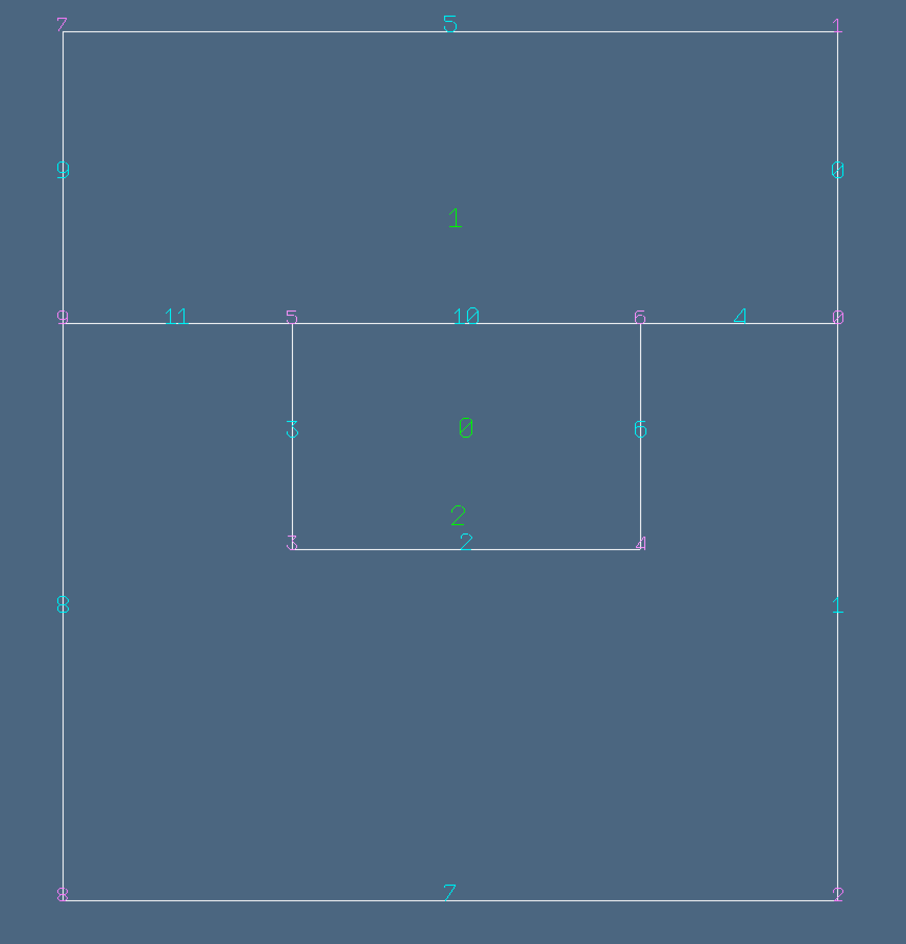
\includegraphics[height=0.245\linewidth,width=0.245\linewidth]{images/boundary-test02-1} 
   
\includegraphics[height=0.245\linewidth,width=0.245\linewidth]{images/boundary-test02-2} 
   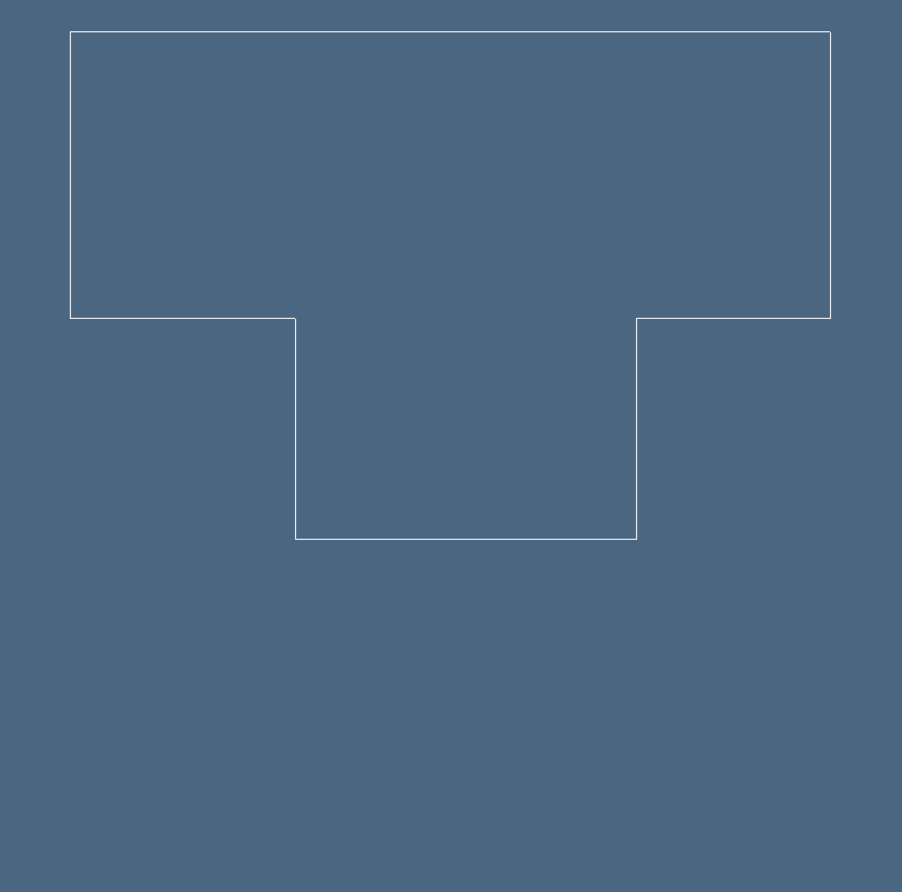
\includegraphics[height=0.245\linewidth,width=0.245\linewidth]{images/boundary-test02-3} 
   
\includegraphics[height=0.245\linewidth,width=0.245\linewidth]{images/boundary-test02-4} 

   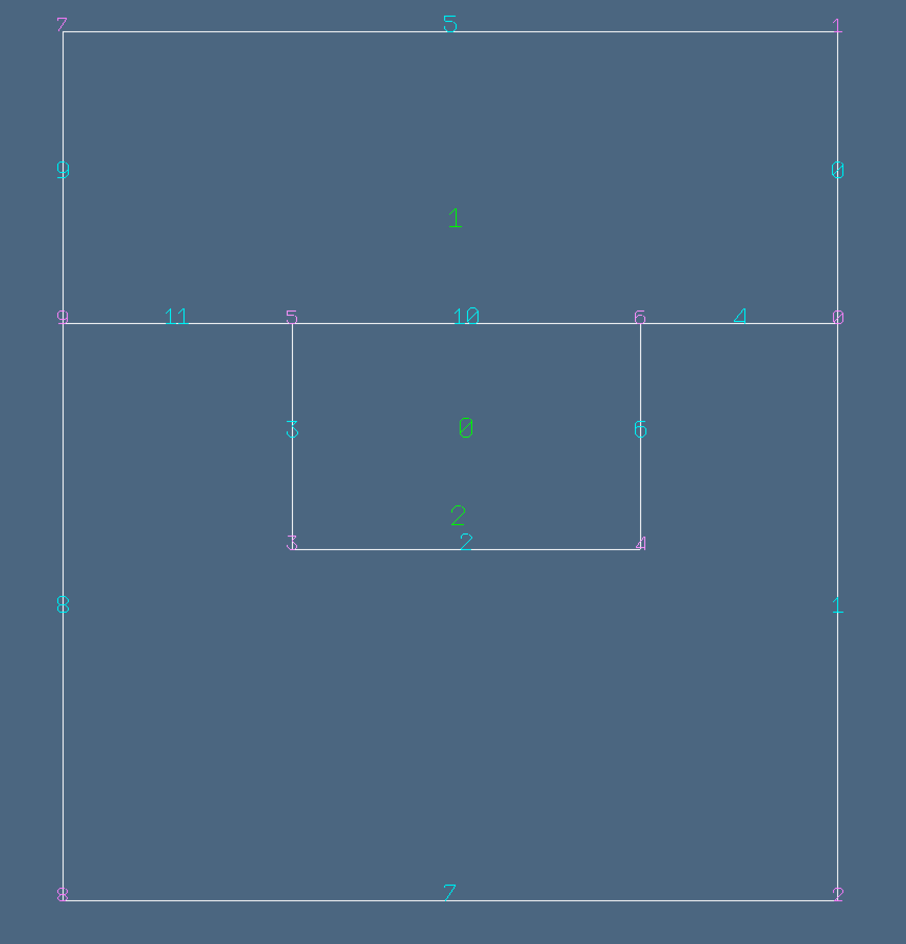
\includegraphics[height=0.245\linewidth,width=0.245\linewidth]{images/boundary-test02-1} 
   
\includegraphics[height=0.245\linewidth,width=0.245\linewidth]{images/boundary-test02-2} 
   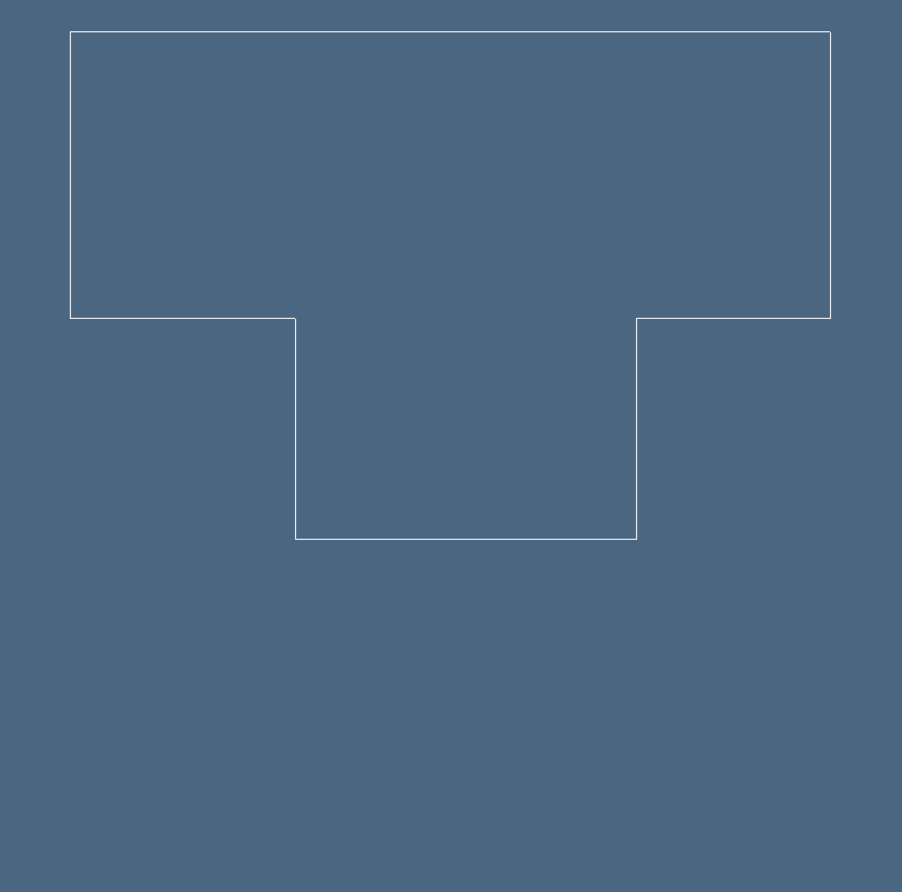
\includegraphics[height=0.245\linewidth,width=0.245\linewidth]{images/boundary-test02-3} 
   
\includegraphics[height=0.245\linewidth,width=0.245\linewidth]{images/boundary-test02-5} 
   \caption{Non-working (i.e.~\emph{wrong}) example with \texttt{boundary}. (a) Indexing of 0-,1-,and 2-cells; (b) boundary of a singleton 2-chain; (c) exploded 2-cells; (d) boundary of a singleton 2-chain. Working (i.e.~\emph{exact}) example using \texttt{boundary1}: (e--h) as above.}
   \label{fig:boundary-test02}
\end{figure}


\paragraph{3D non-convex LAR cells}

%-------------------------------------------------------------------------------
@O test/py/boundary/test03.py
@{""" 3D non-convex LAR cells """
from larlib import *
# LAR model with non-contractible faces
# ------------------------------------------------------------------------------

V = [[0.25, 0.25, 0.0], [0.25, 0.75, 0.0], [0.75, 0.75, 0.0], [0.75, 0.25, 0.0], [1.0, 
0.0, 0.0], [0.0, 0.0, 0.0], [1.0, 1.0, 0.0], [0.0, 1.0, 0.0], [0.25, 0.25, 1.0], [0.25, 
0.25, 2.0], [0.25, 0.75, 2.0], [0.25, 0.75, 1.0], [0.25, 0.75, -1.0], [0.25, 0.25, 
-1.0], [0.75, 0.75, -1.0], [0.75, 0.25, -1.0], [0.75, 0.25, 1.0], [0.75, 0.75, 1.0], 
[1.0, 0.0, 1.0], [0.0, 0.0, 1.0], [1.0, 1.0, 1.0], [0.0, 1.0, 1.0], [0.75, 0.75, 2.0], 
[0.75, 0.25, 2.0]]

CV = [(0,1,2,3,4,5,6,7,8,11,16,17,18,19,20,21), 
(0,1,2,3,8,11,16,17),
(0,1,2,3,12,13,14,15), 
(8,9,10,11,16,17,22,23)]

FV = [(2,3,16,17),(6,7,20,21),(12,13,14,15),(0,1,8,11),(1,2,11,17),(0,1,12,13),
(4,6,18,20),(5,7,19,21),(0,3,13,15),(0,3,8,16),(0,1,2,3),
(10,11,17,22),(2,3,14,15),(8,9,16,23),(8,11,16,17),
(1,2,12,14),(16,17,22,23),(4,5,18,19),(8,9,10,11),(
9,10,22,23),(0,1,2,3,4,5,6,7),(8, 11,16,17,18,19,20,21)]

EV =[(3,15),(7,21),(10,11),(4,18),(12,13),(5,19),(8,9),(18,19),(22,23),(0,3),(1,11),
(16,17),(0,8),(6,7),(20,21),(3,16),(10,22),(18,20),(19,21),(1,2),(12,14),(4,5),(
8,11),(13,15),(16,23),(14,15),(11,17),(17,22),(2,14),(2,17),(0,1),(9,10),(8,16),
(4,6),(1,12),(5,7),(0,13),( 9,23),(6,20),(2,3)]

VV = AA(LIST)(range(len(V)))
hpc = STRUCT(MKPOLS((V,EV)))
VIEW(larModelNumbering(1,1,1)(V,[VV,EV,FV,CV],hpc,0.6))

BF = boundaryCells1(CV,FV,EV)
VIEW(EXPLODE(1.2,1.2,1.2)(MKTRIANGLES((V,[FV[f] for f in BF],EV))))
@}
%-------------------------------------------------------------------------------

\begin{figure}[htbp] %  figure placement: here, top, bottom, or page
   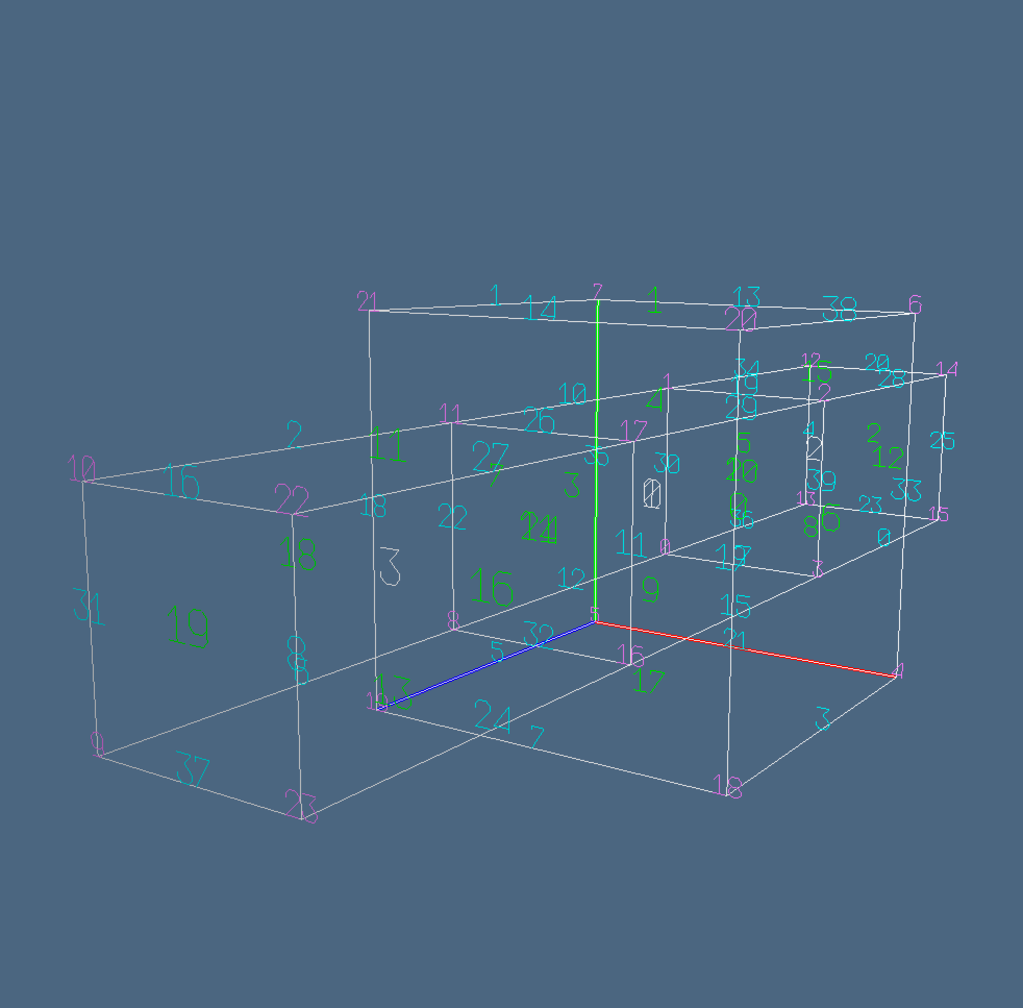
\includegraphics[height=0.495\linewidth,width=0.495\linewidth]{images/boundary-test03-1} 
   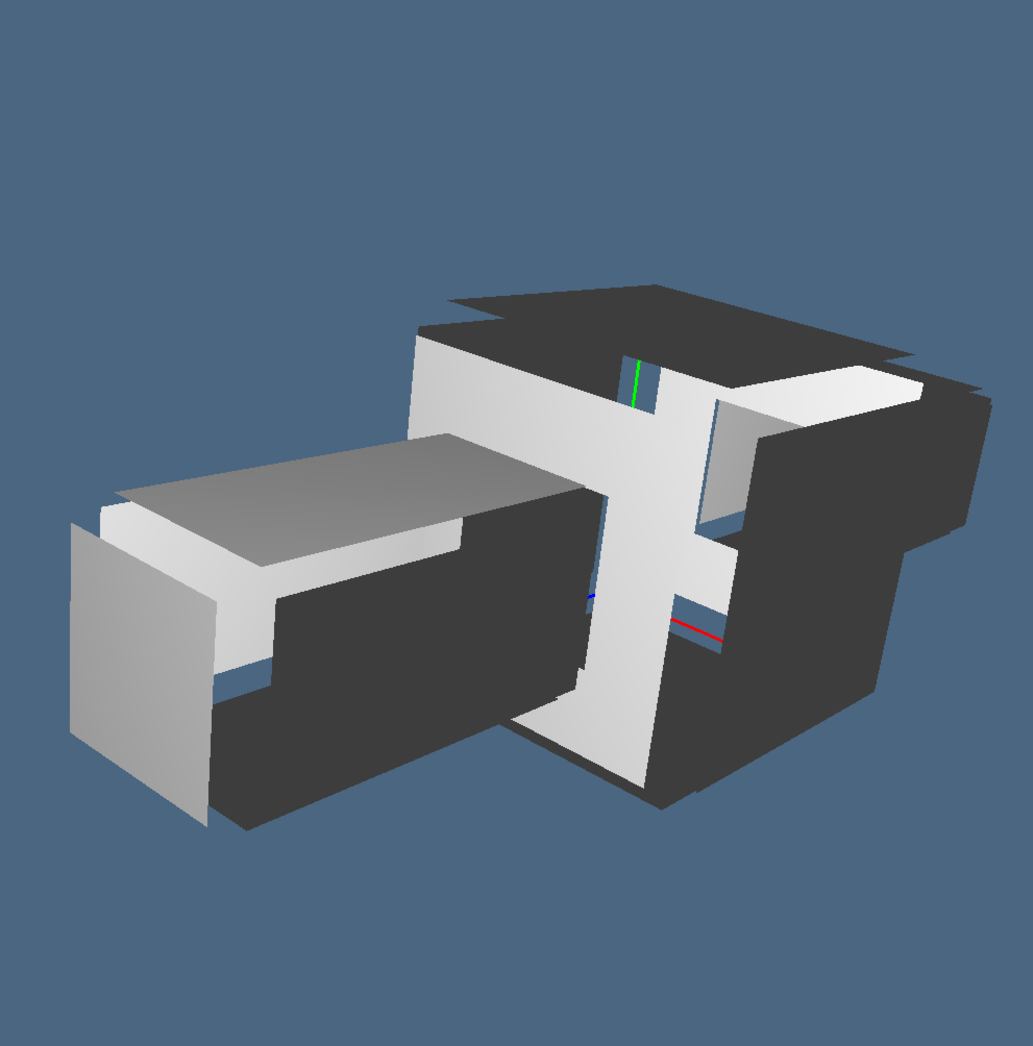
\includegraphics[height=0.495\linewidth,width=0.495\linewidth]{images/boundary-test03-2} 
   \caption{Non-convex 3-complex. (a) Indexing of 0-,1-,2- and 3-cells; (b) exploded 2-boundary cells.
   Notice that two faces are multiply-connected.}
   \label{fig:boundary-test03}
\end{figure}


\bibliographystyle{amsalpha}
\bibliography{boundary}

\end{document}
